%%
% The SUEPThesis Template for Bachelor Graduation Thesis
%
% 上海电力大学毕业设计(论文)中英文摘要 —— 使用 XeLaTeX 编译
%
% Copyright 2020-2023 SUEPaper
%
% This work may be distributed and/or modified under the
% conditions of the LaTeX Project Public License, either version 1.3
% of this license or (at your option) any later version.
% The latest version of this license is in
%   http://www.latex-project.org/lppl.txt
% and version 1.3 or later is part of all distributions of LaTeX
% version 2005/12/01 or later.
%
% This work has the LPPL maintenance status `maintained'.
%
% The Current Maintainer of this work is Haiwen Zhang.
%%

\chapter{未来订单未知情形的WPCR不确定生产和存储模型}

\section{WPCR不确定生产和存储模型的建立}

在该模型中,要求既能够保障每天的WPCR订单均以95\%以上的概率保证正常交付,
又能够以85\%以上的概率保证整周的WPCR订单能正常交付。

设划置信区间,置信区间是95\%,只要假设得到的偏差值大于0.05就说明拒绝原假设,且一周生产计划中保证85\%以上的日交付率,
如一周内至少有一天未正常交付则拒绝原假设。

设$d$为决策变量的函数,正偏差变量$d^+$表示决策值超过目标值的部分,负偏差变量$d^-$表示决策值未达到目标值的部分,
这里$d0$表示$d$的目标值。
\begin{equation}
    d^+=\max\{d-d_0,0\}
\end{equation}
\begin{equation}
    d^-=-\min\{d-d_0,0\}
\end{equation}

因决策值不可能既超过目标值同时又未达到目标值,即恒有
\begin{equation}
    d^+ \times d^- = 0
\end{equation}

设$x_k(k=1,2,...,n)$是目标规划的决策变量。设有$q$个优先级别,分别为$P_1,P_2,...,P_q$。
在同一个优先级$P$中,有不同的权重,分别记为$w_{kj}^+, w_{kj}^-(j=1,2,...,l)$。
因此目标规划模型的一般数学表达式为
\begin{equation}
    \min z=\sum_{k=1}^{q}P_k(\sum_{l}^{j=1}w_{kj}^-d_{j}^- + w_{kj}^+d_{j}^+)
\end{equation}
\begin{equation}
    \begin{cases}
        \min\sum_{k=1}^{n}(
            C_{\uppercase\expandafter{\romannumeral1}}^{'''}+
            C_{\uppercase\expandafter{\romannumeral2}}^{'''}+
            C_{\uppercase\expandafter{\romannumeral3}}^{'''}) \\
        x_k \geqslant 0 \\
        d_i^-,d_i^+\geqslant 0,i=1,2,...,l
    \end{cases}
\end{equation}

\section{WPCR不确定生产和存储模型的求解}

\subsection{WPCR不确定生产和存储模型的求解算法}

已经有研究表明策略迭代算法可以在适当的假设下产生最优(最小)成本、最优稳态控制策略和平均成本最优方程的解,且有比较好的效果。
因此本模型采用策略迭代算法进行求解。

下面给出策略迭代算法的具体实现步骤。

步骤一:初始化,$i=0$,选择初始容许控制策略。

步骤二:策略评估,$i=i+1$,控制策略$u^{i-1}$下的值函数$V^i$可以根据以下公式获得
\begin{equation}
    L(x,u^{i-1}) + (\nabla V)^{iT}(f(x)+g(x)u^{i-1})=0
\end{equation}

步骤三:策略提升,更新后的控制策略$u^i$如下
\begin{equation}
    u^i=-w(u)g^T(x)\nabla V^i
\end{equation}

步骤四:判断,若策略不满足收敛条件,那么返回步骤二继续执行,否则进入步骤五。

步骤五:结束,获得最优控制策略$u^*=u^i$和最优值函数$V^*=V^i$。
汇总上述五步,得如下策略迭代算法模拟流程图\ref{f.ch5-1}\cite{叶帅2021基于事件触发自适应动态规划的多四旋翼无人机优化控制}。

\begin{figure}[h]
    \centering
    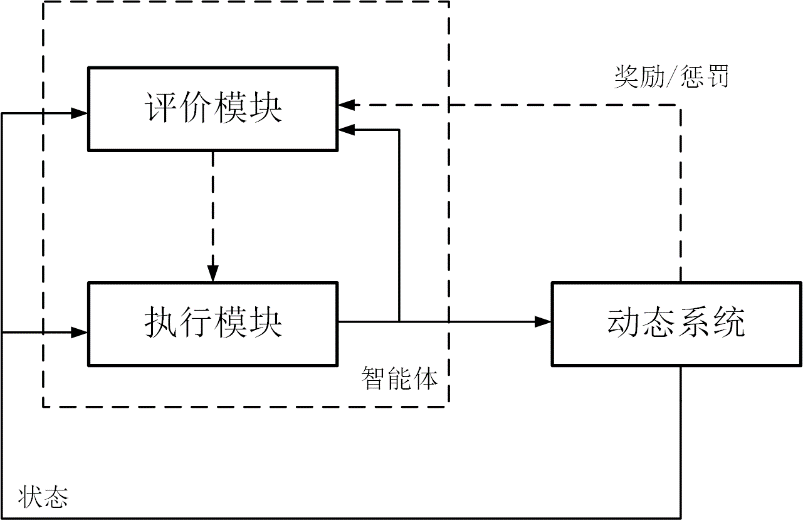
\includegraphics[width=0.5\linewidth]{ch5-1.png}
    \caption{迭代费用对比}
    \label{f.ch5-1}
\end{figure}

\subsection{WPCR不确定生产和存储模型的求解结果}

\begin{table}[H]
    \caption{WPCR不确定生产和存储模型求解的结果}
    \label{T.ch5-1}
    \centering
    \renewcommand\arraystretch{1.5} 
    \begin{tabular}{@{}ccccccc@{}} 
    \toprule
    \textbf{日期} & \multicolumn{1}{c}{\textbf{WPCR外部}} & \multicolumn{1}{c}{\textbf{A组装}} 
    & \multicolumn{1}{c}{\textbf{B组装}} & \multicolumn{1}{c}{\textbf{C组装}}
    & \multicolumn{1}{c}{\textbf{生产准备}} & \multicolumn{1}{c}{\textbf{库存}} \\
                & \multicolumn{1}{c}{\textbf{需求数量}} & \multicolumn{1}{c}{\textbf{数量}} 
    & \multicolumn{1}{c}{\textbf{数量}} & \multicolumn{1}{c}{\textbf{数量}}
    & \multicolumn{1}{c}{\textbf{费用}} & \multicolumn{1}{c}{\textbf{费用}} \\
    \midrule
    \textbf{周一} & 237 & 316 & 395 & 41 & 700 & 1619.5 \\
    \textbf{周二} & 237 & 316 & 395 & 41 & 700 & 1619.5 \\
    \textbf{周三} & 237 & 316 & 395 & 41 & 700 & 1619.5 \\
    \textbf{周四} & 237 & 316 & 395 & 41 & 700 & 1619.5 \\
    \textbf{周五} & 237 & 316 & 395 & 41 & 700 & 1619.5 \\
    \textbf{周六} & 237 & 316 & 395 & 41 & 700 & 1619.5 \\
    \textbf{周日} & 237 & 316 & 395 & 41 & 700 & 1619.5 \\
    \textbf{总和} & 237 & 316 & 395 & 41 & 700 & 1619.5 \\ 
    \bottomrule
    \end{tabular}
\end{table}

从表\ref{T.ch5-1}可以看出,该模型下,一周里面每天都有生产计划,不至于出现前几种模型中出现无生产计划的情况。